
%!TEX root = ../main.tex
\section{Activation energy of Si}
The activation energy of Si can be determined from the electrical conductivity $\sigma$. For this applies:

\begin{align}
    &\sigma = \frac{1}{\rho} = \frac{l}{R\cdot A} \
    &\sigma = C\cdot \exp \left (\frac{-E_a}{2k_BT} \right ) 
\end{align}

where l is the length and A is the cross-sectional area of the sample. For the silicon semiconductor, it follows:
\begin{align}
    \Rightarrow ln\left( \frac{1}{R}\right ) = \frac{-E_a}{2k_B} \cdot \frac{1}{T} -ln \left ( \frac{l}{AC} \right )
\end{align}
Therefore, if we plot the natural logarithm of the inverse resistance versus the inverse temperature, we can see a linear relationship at low temperatures. Hence, from the fit $f(x) = Ax+B $, the activation energy can be determined. 
\begin{figure}
    \centering
    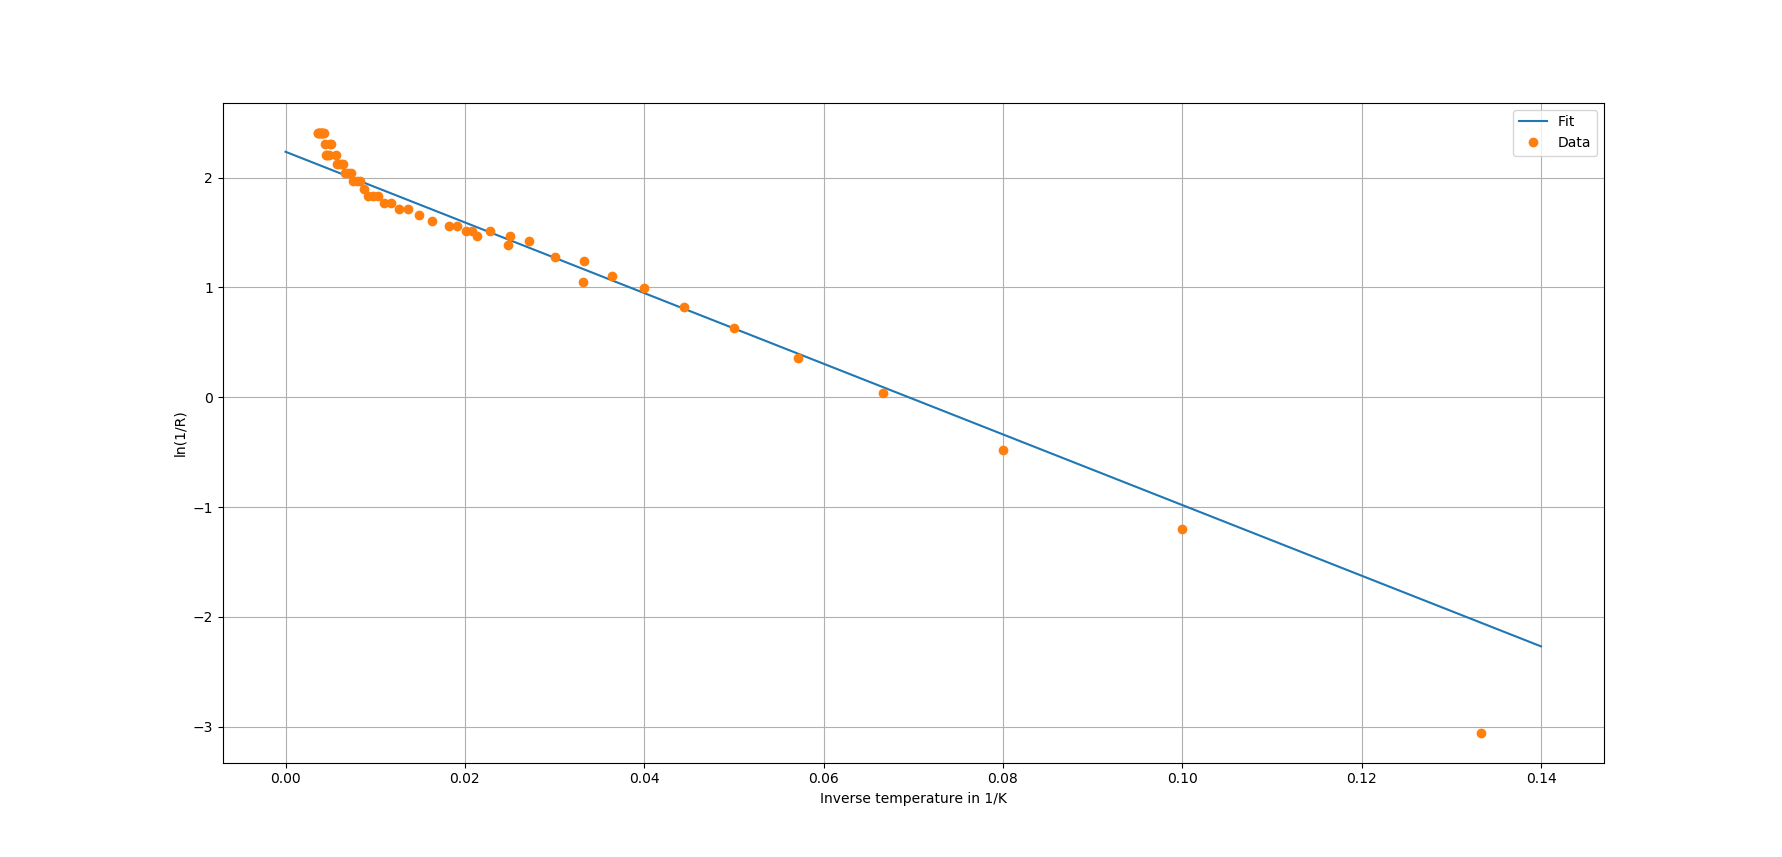
\includegraphics[width=1.0\textwidth]{./fig/ex4.1.png}
    \caption{Fit for the activation energy}
    \label{fig:E_activation}
\end{figure}
As for the activation energy with gradient $A = \SI{-32,17\pm1,02}{K}$:
\begin{align}
    E_a &= -2k_BA &k_B = \SI{8,617343}{\frac{eV}{K}} \\
    \Rightarrow E_a &= \SI{5,54\pm 0,18}{meV}
\end{align}